\section{Applications}

\subsection{Denoising}

\begin{description}
 \item[btkNLMDenoising] This program applies a non-local mean filter to a 3D image for denoising purpose. Usage: \texttt{-i input\_image\_filename -o output\_image\_filename}. The best results are usually obtained by using a mask (or a padding value).
\end{description}

\begin{description}
 \item[btkNLMDenoising4DImage] This program applies a non-local mean filter to each 3D image of a 4D image, for denoising purpose. Usage: \texttt{-i input\_image\_filename -o output\_image\_filename}. The best results are usually obtained by using a mask (or a padding value).
\end{description}


\subsection{Anatomical reconstruction}

\begin{description}
 \item[btkImageReconstruction] This program allows to obtain a
high-resolution image from a set of low-resolution images, typically
axial, coronal, and sagital acquisitions~\cite{Rousseau2006}. \\\\
Minimal usage: \texttt{btkImageReconstruction -i image1 $\cdots$ -i imageN -o
output --box}. 

Recommended usage: \texttt{btkImageReconstruction -i image1 $\cdots$ -i imageN
-m mask1 $\cdots$ -m maskN -o output --mask}. The use of a mask provide
better results since it allows an accuratelly estimation of the initial
transform, and constrains the registration to the region of interest.

The full list of optional parameters of the method can be obtained by
\texttt{btkImageReconstruction --help}

\end{description}

\subsection{Tractography}

    \subsubsection*{Standard usage}
        Suppose you want to perform a tractography on a diffusion weighted MRI dataset. You should have a dwi image, the corresponding gradient vectors' coordinates, a mask of the brain white matter and a label image of the seeds. Assume this data is stored in files named repsectively for instance \texttt{data.nii.gz}, \texttt{data.bvec}, \texttt{mask.nii.gz} and \texttt{seeds.nii.gz}. The tractography is accomplished by the command below.
            \begin{quote}
                \texttt{btkTractography -d data.nii.gz -v data.bvec -m mask.nii.gz -l seeds.nii.gz}
            \end{quote}
        When the program terminates its task, the probability connection map and the fibers estimation are saved in files respectively named \texttt{map.nii.gz} and \texttt{fibers.vtk}. The connection map is a volume image of probability intensities (\texttt{i.e.} intensities between 0 and 1) with the same origin, orientation and spacing as the diffusion weighted image. The fibers are polygonal data of VTK library in world coordinates. The standard pipeline of the program is shown in Fig.~\ref{btkTractography-fig:standard-pipeline}.
            \begin{figure}
                \centering
                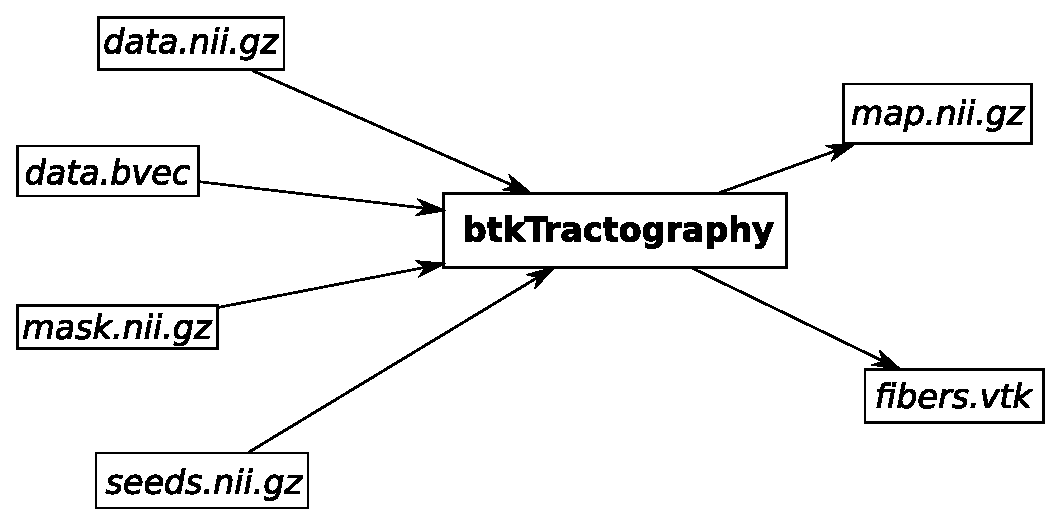
\includegraphics[width=0.6\textwidth]{btkTractographyPipeline}
                \caption{Standard pipeline of the btkTractography program.}
                \label{btkTractography-fig:standard-pipeline}
            \end{figure}

    \subsubsection*{Advanced usage}
        In addition to standard arguments of \texttt{btkTractography} program, there are some other parameters that let you to alter algorithm's behaviour. These options can be classified into three groups : model's options, constraints on trajectory and filter's options. The first group options allow you to tweak the model (for more details about it, please refer to~\cite{descoteaux_regularized_2007}). The second group options let you to control the particle's trajectory. These options provide prior informations to the algorithm. The last group options are dedicated to the particle filter control.

        Since the default parameters values may work in the most of cases, they are optional. A list is of optional features is avaible by using the command
            \begin{quote}
                \texttt{btkTractography -\hspace{0.1mm}-help}
            \end{quote}
        and program's arguments are much more described below.


    \subsubsection*{Model's order}
        The model's order (i.e. the spherical harmonics' order) can be specified by the option
            \begin{quote}
                \texttt{-\hspace{0.1mm}-model\_order <order>} \enspace ,
            \end{quote}
        for \texttt{order}$\;\in\{2,4,6,8\}$. The default value is 4. For more details, please refer to~\cite{descoteaux_regularized_2007}.

    \subsubsection*{Model's regularization}
        A Laplace-Beltrami regularization coefficient is used to assume a better estimation of the model. This coefficient can by manually modified by the option
            \begin{quote}
                \texttt{-\hspace{0.1mm}-model\_regularization <coefficient>} \enspace ,
            \end{quote}
        for \texttt{coefficient}$\;\in\mathbb{R}$. The default value is set as 0.006. For more details, please refer to~\cite{descoteaux_regularized_2007}.

    \subsubsection*{Displacement step size}
        The displacement step size of a moving particle can ben adjusted as you want by using the option
            \begin{quote}
                \texttt{-\hspace{0.1mm}-step\_size <length>} \enspace ,
            \end{quote}
        where \texttt{length}$\;\in\mathbb{R}_+^*$. Note that this option is expressed in the voxel unit. The default value is fixed at 0.5 voxel.
        By setting a big step size, the particles will move quickly. So the biger is the step, the faster the algorithm will finish, but as shown by Fig.~\ref{tracto-fig:stepSize}, some informations may be missed and the particle's trajectories may overshoot the ground truth, resulting in a bad estimation.

        \begin{figure}
            \centering
            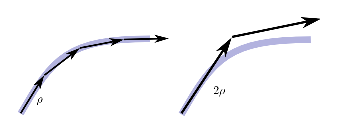
\includegraphics[height=0.1\textheight]{stepSize}
            \caption{Effect of the step size option on a particle's trajectory. With a large step size (right), the particle may overshoot the trajectory of the ground truth.}
            \label{tracto-fig:stepSize}
        \end{figure}


    \subsubsection*{Angular threshold}
        An angular threshold prevent a particle to return back. This option has to be expressed in radian and can bet set by
            \begin{quote}
                \texttt{-\hspace{0.1mm}-angular\_threshold <angle>} \enspace ,
            \end{quote}
        where \texttt{angle}$\;\in]0,2\pi[$. The default value is set as a $\tfrac{\pi}{3}$ angle.
        As illustrated in two dimensions in Fig.~\ref{tracto-fig:angleThreshold}, an angle threshold is used to define an allowed area for successive sampled directions. This can be seen as a global curvature parameters on trajectories. A small angle defines trajectories with a small curvature. This is a prior information on ground truth trajectory.

        \begin{figure}
            \centering
            
\includegraphics[height=0.1\textheight]{angleThreshold}
            \caption{An angle threshold allows the algorithm to sample successive direction only in the cone defined by this angle. This illustration show the principle in two dimensions.}
            \label{tracto-fig:angleThreshold}
        \end{figure}


    \subsubsection*{Rigidity}
        The rigidity option controls how much you want the particles to have straight trajectory. You can adjust it by
            \begin{quote}
                \texttt{-\hspace{0.1mm}-curve\_constraint <rigidity>} \enspace ,
            \end{quote}
        where \texttt{rigidity}$\;\in\mathbb{R}_+^*$. The default value is fixed at 30.
        This value correspond to a concentration parameter of a von Mises-Fisher density probability used in the prior density of the system. As Fig.~\ref{tracto-fig:concentration} illustrates locally in two dimensions, a high value leads to a straight trajectory.

        \begin{figure}
            \centering
            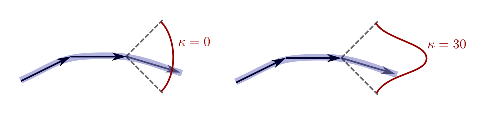
\includegraphics[height=0.1\textheight]{concentration}
            \caption{Local effect of rigidity parameter on a particle's trajectory. This parameter helps to ``attract'' the current displacement vector in the direction of the previous displacement vector of a particle. It correspond to a concentration paramter of a von Mise-Fisher density probability used in the prior density of the system. For instance, a rigidity of 0 leads to an equiprobable distribution, whereas a rigidty tending to infinity leads to a distribution focused on a point.}
            \label{tracto-fig:concentration}
        \end{figure}


    \subsubsection*{Number of particles}
        The number of particles in the system is set by the option
            \begin{quote}
                \texttt{-\hspace{0.1mm}-number\_of\_particles <number>} \enspace ,
            \end{quote}
        where \texttt{number}$\;\in\mathbb{N}^*$. By default, the algorithm will use 1000 particles.
        A poor number of particles leads to a short computation time and a poor estimation. A large number of particles leads to a long computation time and a good estimation. In general, the default number of particles is a good compromise between computation time and estimation.


    \subsubsection*{Resampling threshold}
        This option modify the resampling threshold of the system. When the number of effective particles in the system falls below this resampling threshold, the particles are resampled according a multinomial resampling. It can be adjust by
            \begin{quote}
                \texttt{-\hspace{0.1mm}-resampling\_threshold <percent>} \enspace ,
            \end{quote}
        where \texttt{percent}$\;\in[0,1]$ is the percent of minimal effective particles in the system.
        A low threshold value will result in an inefficient algorithm because the particles with low weight are not are not often eliminated. Conversely, a high threshold value leads to a bad estimation because the search space will not be explored enough.
